%
% strahlensatz.tex
%
% (c) 2018 Prof Dr Andreas Müller, Hochschule Rapperswil
%
\documentclass[tikz]{standalone}
\usepackage{times}
\usepackage{amsmath}
\usepackage{txfonts}
\usepackage[utf8]{inputenc}
\usepackage{graphics}
\usetikzlibrary{arrows,intersections}
\begin{document}
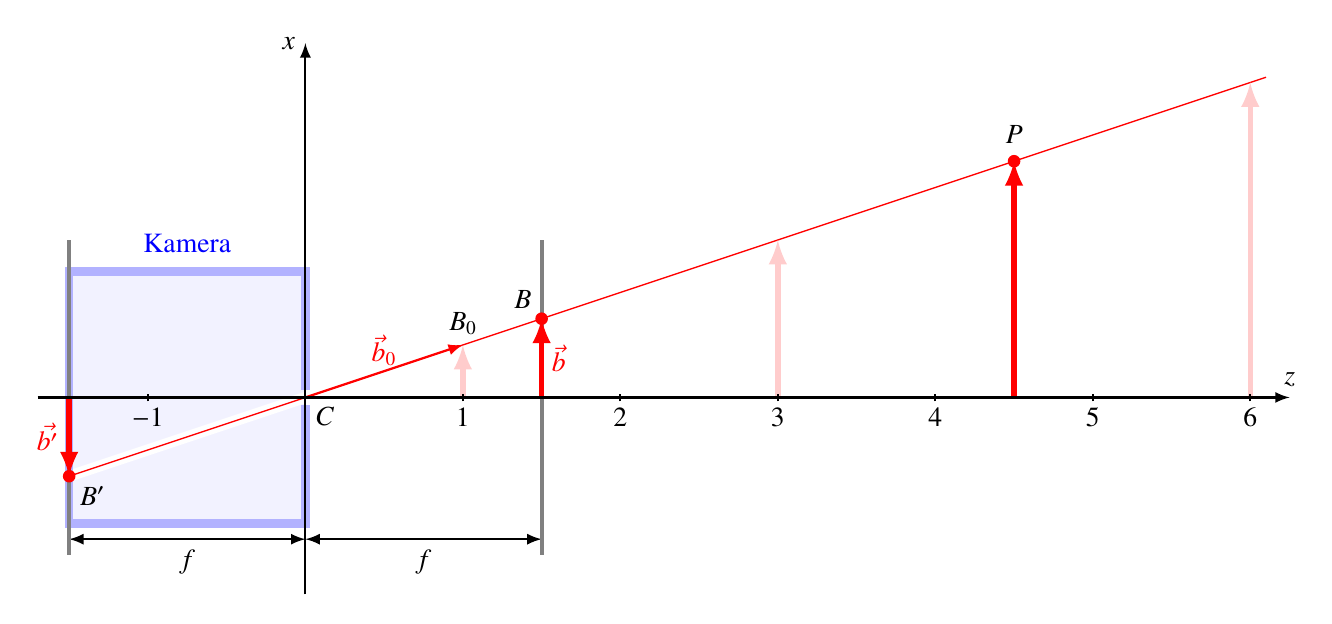
\begin{tikzpicture}[>=latex,thick]

\fill[color=blue!5] (-3,-1.6) rectangle (0,1.6);
\draw[color=white,line width=4pt] (0,0)--(-3.1,{-3.1/3});
\draw[color=blue!30,line width=3pt] (0,-0.1)--(0,-1.6)--(-3,-1.6)--(-3,1.6)--(0,1.6)--(0,0.1);

\node[color=blue] at (-1.5,1.7) [above] {Kamera};

\draw[<->] (-3,-1.8)--(0,-1.8);
\draw[<->] (3,-1.8)--(0,-1.8);
\node at (-1.5,-1.8) [below] {$f$};
\node at (1.5,-1.8) [below] {$f$};

\node at (3,1) [above left] {$B$};
\node at (-3,-1) [below right] {$B'$};

\draw[color=gray,line width=1.5pt] (-3,-2)--(-3,2);
\draw[color=gray,line width=1.5pt] (3,-2)--(3,2);

\draw[color=red, line width=0.5pt] (12.2,{4*12.2/12})--(-3,-1);
\draw[->,color=red,line width=2pt] (9,0)--(9,3);
\draw[->,color=red!20,line width=2pt] (12,0)--(12,4);
\draw[->,color=red!20,line width=2pt] (6,0)--(6,2);
\draw[->,color=red,line width=2pt] (3,0)--(3,1);
\node[color=red] at (3,0.5) [right] {$\vec{b}$};
\draw[->,color=red,line width=2pt] (-3,0)--(-3,-1);
\node[color=red] at (-3,-0.5) [left] {$\vec{b'}$};

\draw[->,color=red!20,line width=2pt] (2,0)--(2,{2/3});
\node[color=red] at (1,{1/6+0.1}) [above] {$\vec{b}_0$};
\draw[->,color=red] (0,0)--(2,{2/3});
\node at (2,{2/3}) [above] {$B_0$};

\foreach \x in {1,2,...,6}{
	\draw ({\x*2},-0.05)--({\x*2},0.05);
	\node at ({\x * 2},0) [below] {$\x$};
}
\draw (-2,-0.05)--(-2,0.05);
\node at (-2,0) [below] {$-1$};

\fill[color=red] (9,3) circle[radius=0.08];
\fill[color=red] (3,1) circle[radius=0.08];
\fill[color=red] (-3,-1) circle[radius=0.08];
\node at (9,3.1) [above] {$P$};

%\node at (9,1.5) [right] {$x(z)$};
\draw (9,-0.01)--(9,0.01);
%\node at (9,0) [below] {$\mathstrut z$};

\node at (0,0) [below right] {$C$};

\draw[->] (-3.4,0)--(12.5,0) coordinate[label=$z$];
\draw[->] (0,-2.5)--(0,4.5) coordinate[label={left:$x$}];

\end{tikzpicture}
\end{document}
